\lecture{2}{Mon 09 Mar 2020 13:41}{Definizione e Classificazione}{

\begin{itemize}
	\item Segni: indicatori di malattia osservabili
	\item Sintomi: percezione soggettiva di malessere
	\item Sindrome: covariazione di sintomi/segni, eziologia non nota
	\item Malattia: sindrome con eziologia, prognosi e decorso noti e caratteristici
\end{itemize}

In psicopatologia le l'eziologia è sempre multi fattoriale.
\medskip\\
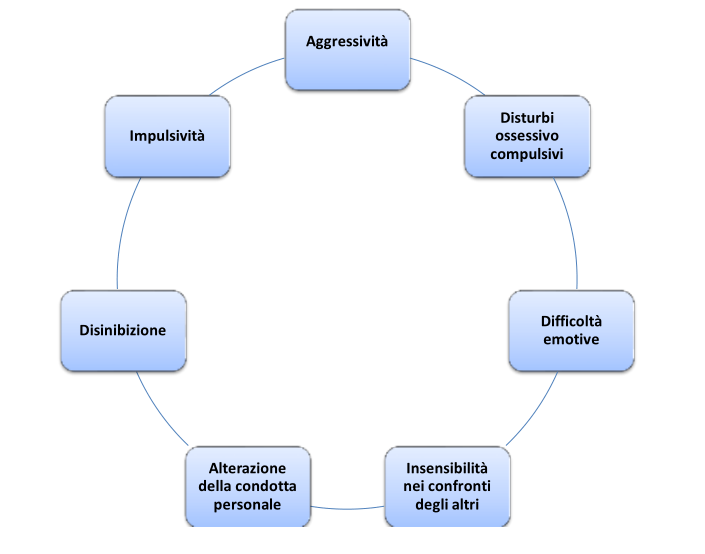
\includegraphics[width=\linewidth]{./images/image2}
\medskip\\

Secondo la visione biopsicosociale ci sono fattori:

\begin{itemize}
	\item Predisponenti
	\item Precipitanti
	\item Perpetuanti (di mantenimento) 
	\item Protettivi
\end{itemize} 
\begin{quote}
	\emph{ “La malattia mentale potrebbe (o dovrebbe) essere definita solo in presenza di dati quali: un’eziologia accertata (conoscenza delle cause e dei fattori che favoriscono o inibiscono il processo morboso); corrispondenti reperti anatomo-biologici; e rilievi patogenetici (correlazioni dimostrabili tra cause, reperti biologici ed effetti sintomatologici obiettivabili)”. }
	\begin{flushright}
		Gilberti et al., 1996
	\end{flushright}
\end{quote}

In realtà non abbiamo informazioni sulla malattia:
\medskip\\

\includegraphics[width=\linewidth]{./images/image1}
\medskip\\
Ovviamente la diagnosi non è altro che un'etichetta, un nome comune, come \emph{giraffa}, che ci dà però informazioni molto precise.

La definizione del DSM-5 del disturbo mentale è: 
\medskip\\

\includegraphics[width=\linewidth]{./images/image3}
\medskip\\
Un disturbo mentale è una sindrome caratterizzata da un’alterazione clinicamente significativa della sfera cognitiva, della regolazione delle emozioni o del comportamento di un individuo, che riflette una disfunzione nei processi psicologici, biologici o evolutivi che sottendono il funzionamento mentale.
